\documentclass[a4paper]{article}

\usepackage{comment} % enables the use of multi-line comments (\ifx \fi) 
\usepackage{lipsum} %This package just generates Lorem Ipsum filler text. 
\usepackage{fullpage} % changes the margin
\usepackage{graphicx}
\usepackage{float}
\graphicspath{.}

\title{Mean Field Inference}

\author{Yu Che Wang / yuchecw2}

\date{\today}

\begin{document}
\maketitle
\section{Introduction}
In this project, I used the MNIST dataset to implement Mean Field Inference. I performed 3 operations on each image: 1. Binarize by mapping any value below 0.5 to -1 and any value above to 1 2. Add noise randomly by flipping 2\% of the bits 3. Denoise using Boltzman machine model and mean field inference.

\section{Average accuracy}
The accuracy for each denoised image is obtained by calculating the ratio of pixels with correct value. The average accuracy on first 500 images is 0.9836.

\section{Sample images}
\begin{figure}[H]
\centering
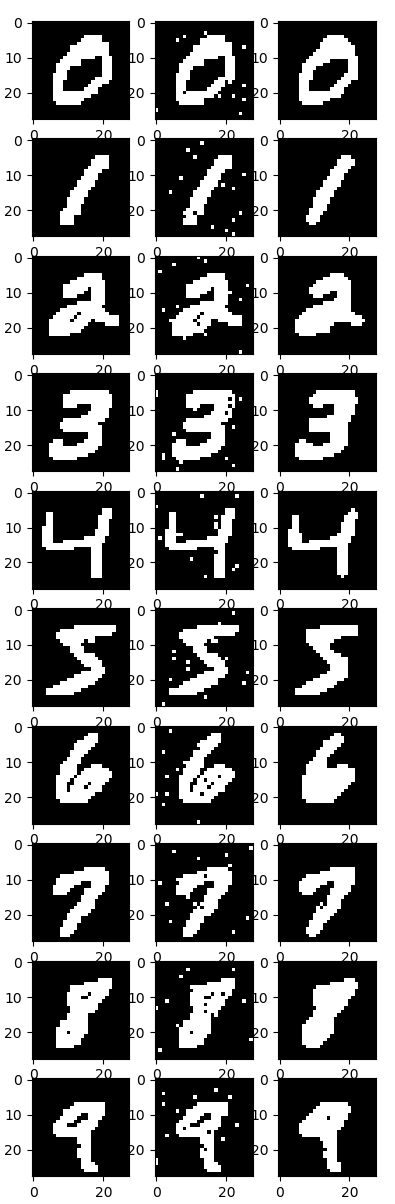
\includegraphics[width=0.23\textwidth]{samples.png}
\caption{\label{fig:data}Sample images for each digit. The first column is sample image, the second column is noised version, and the third column is denoised version.}
\end{figure}

\section{Best reconstruction}
\begin{figure}[H]
\centering
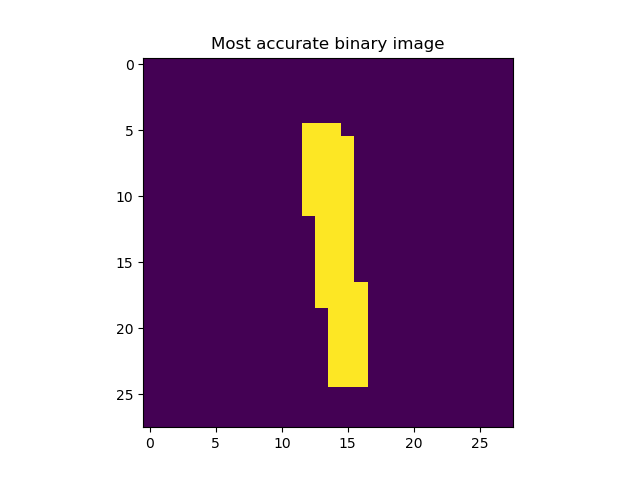
\includegraphics[width=0.3\textwidth]{most_accurate_binary_image.png}
\caption{\label{fig:data}Original image of the best reconstruction}
\end{figure}
\begin{figure}[H]
\centering
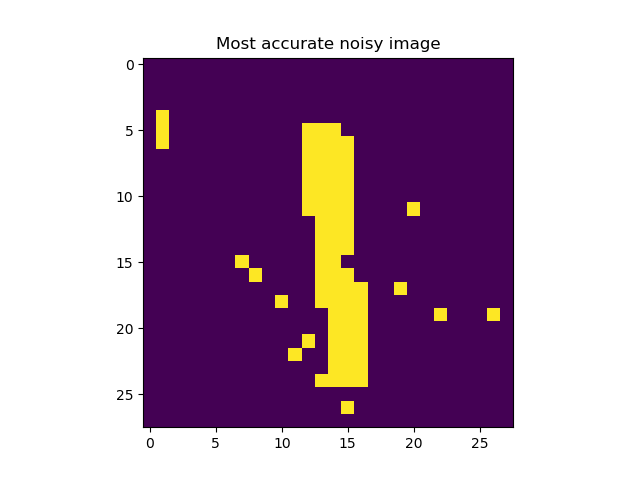
\includegraphics[width=0.3\textwidth]{most_accurate_noisy_image.png}
\caption{\label{fig:data}Noised version of the best reconstruction}
\end{figure}
\begin{figure}[H]
\centering
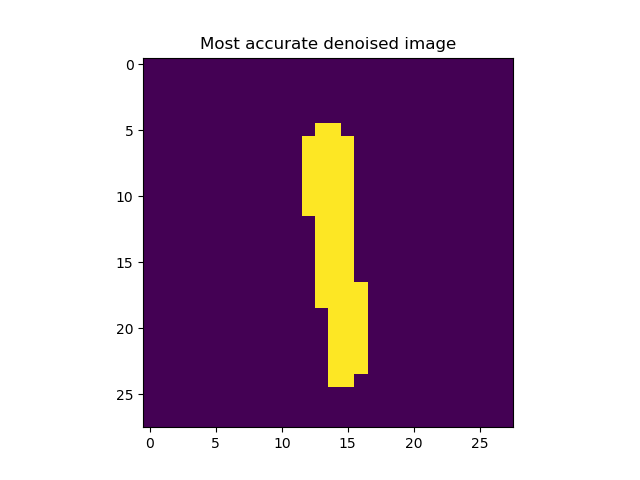
\includegraphics[width=0.3\textwidth]{most_accurate_denoised_image.png}
\caption{\label{fig:data}Denoised version of the best reconstruction}
\end{figure}

\section{Worst reconstruction}
\begin{figure}[H]
\centering
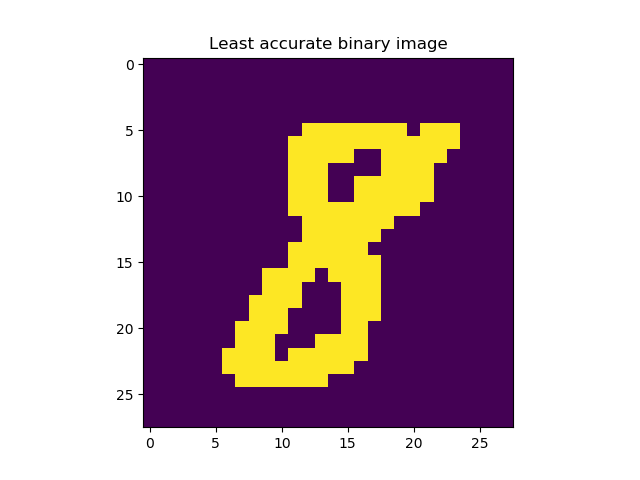
\includegraphics[width=0.3\textwidth]{least_accurate_binary_image.png}
\caption{\label{fig:data}Original image of the worst reconstruction}
\end{figure}
\begin{figure}[H]
\centering
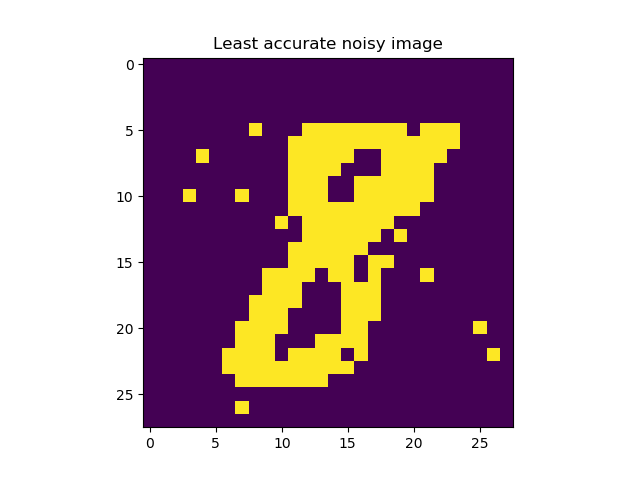
\includegraphics[width=0.3\textwidth]{least_accurate_noisy_image.png}
\caption{\label{fig:data}Noised version of the worst reconstruction}
\end{figure}
\begin{figure}[H]
\centering
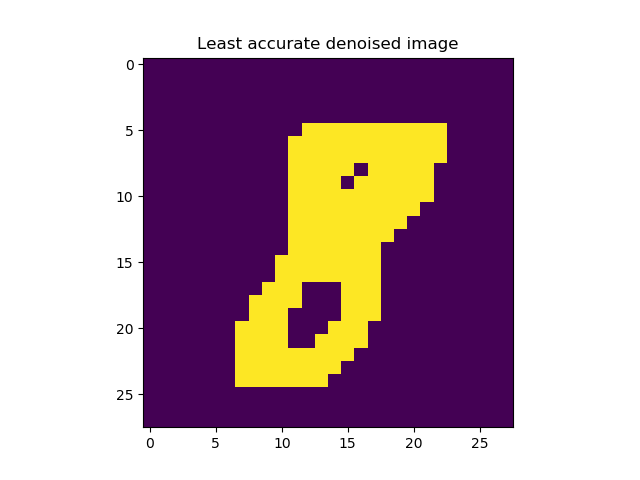
\includegraphics[width=0.3\textwidth]{least_accurate_denoised_image.png}
\caption{\label{fig:data}Denoised version of the worst reconstruction}
\end{figure}

\section{ROC Curve}
\begin{figure}[H]
\centering
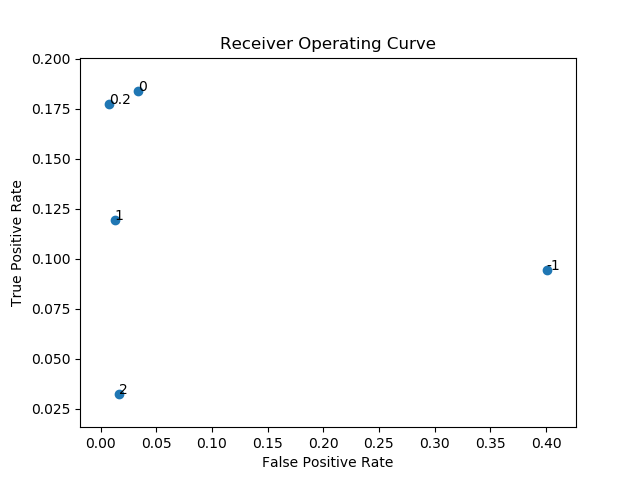
\includegraphics[width=0.9\textwidth]{roc.png}
\caption{\label{fig:data}Receiver operating curve. The label for each data point is the value of $\theta_{ij}$ for the $H_i$, $H_j$ terms.}
\end{figure}

\section{Code}
\subsection{Helper functions}
\begin{figure}[H]
\centering
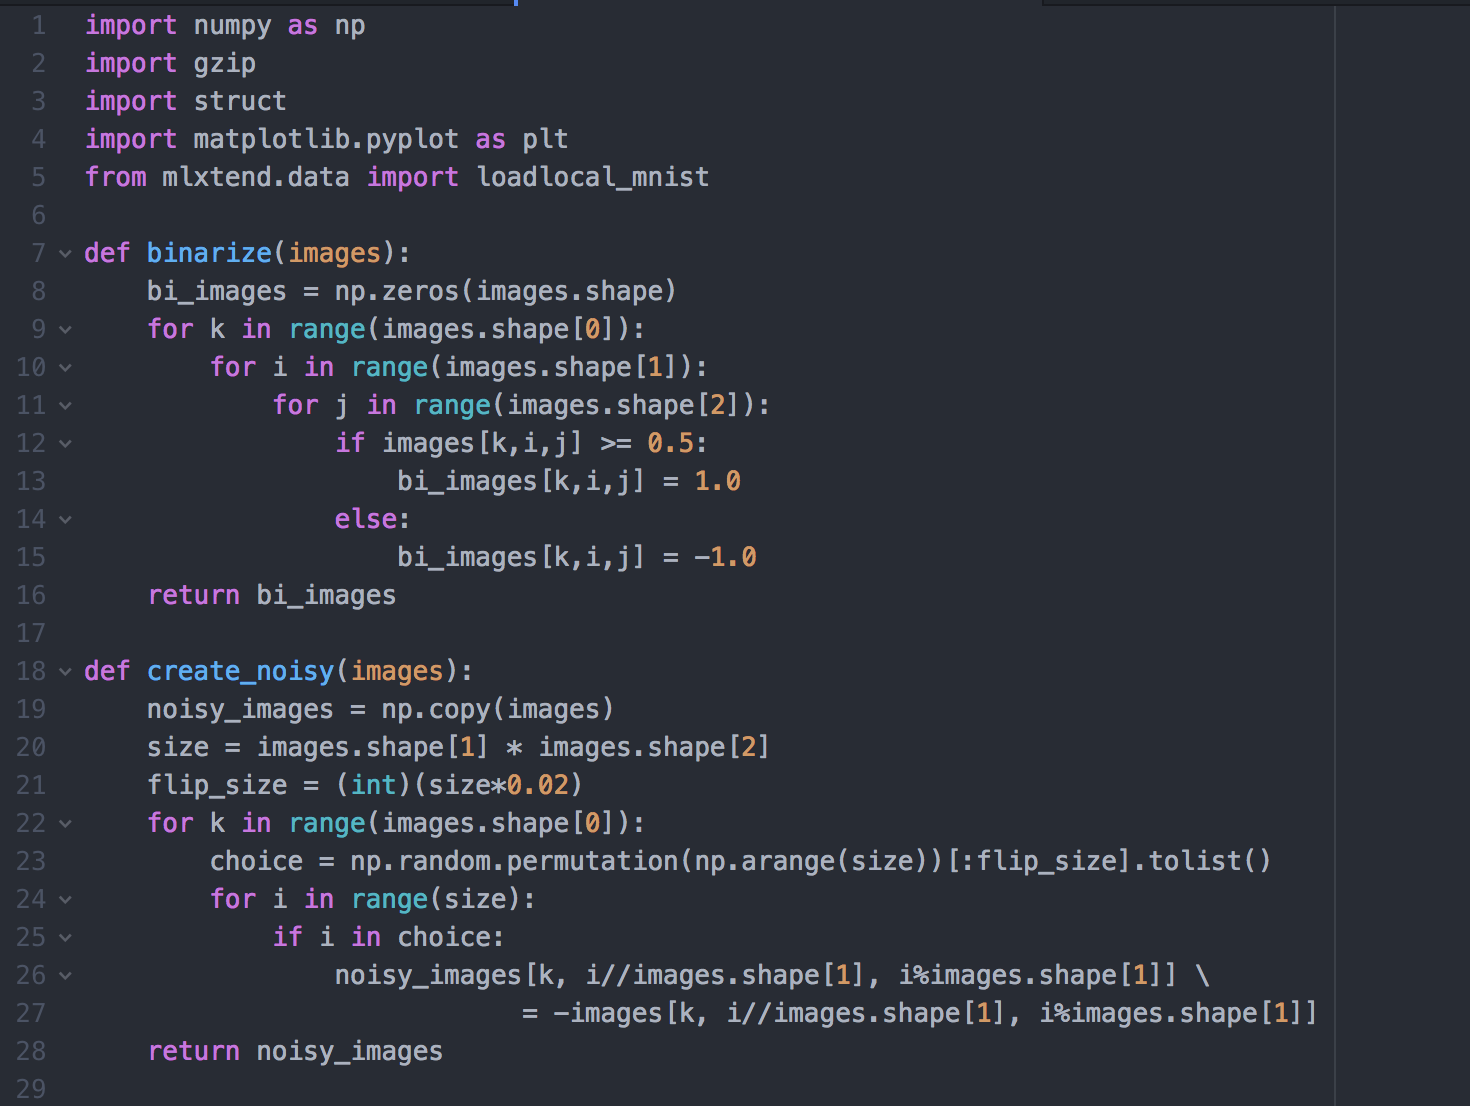
\includegraphics[width=1\textwidth]{1.png}
\end{figure}
\begin{figure}[H]
\centering
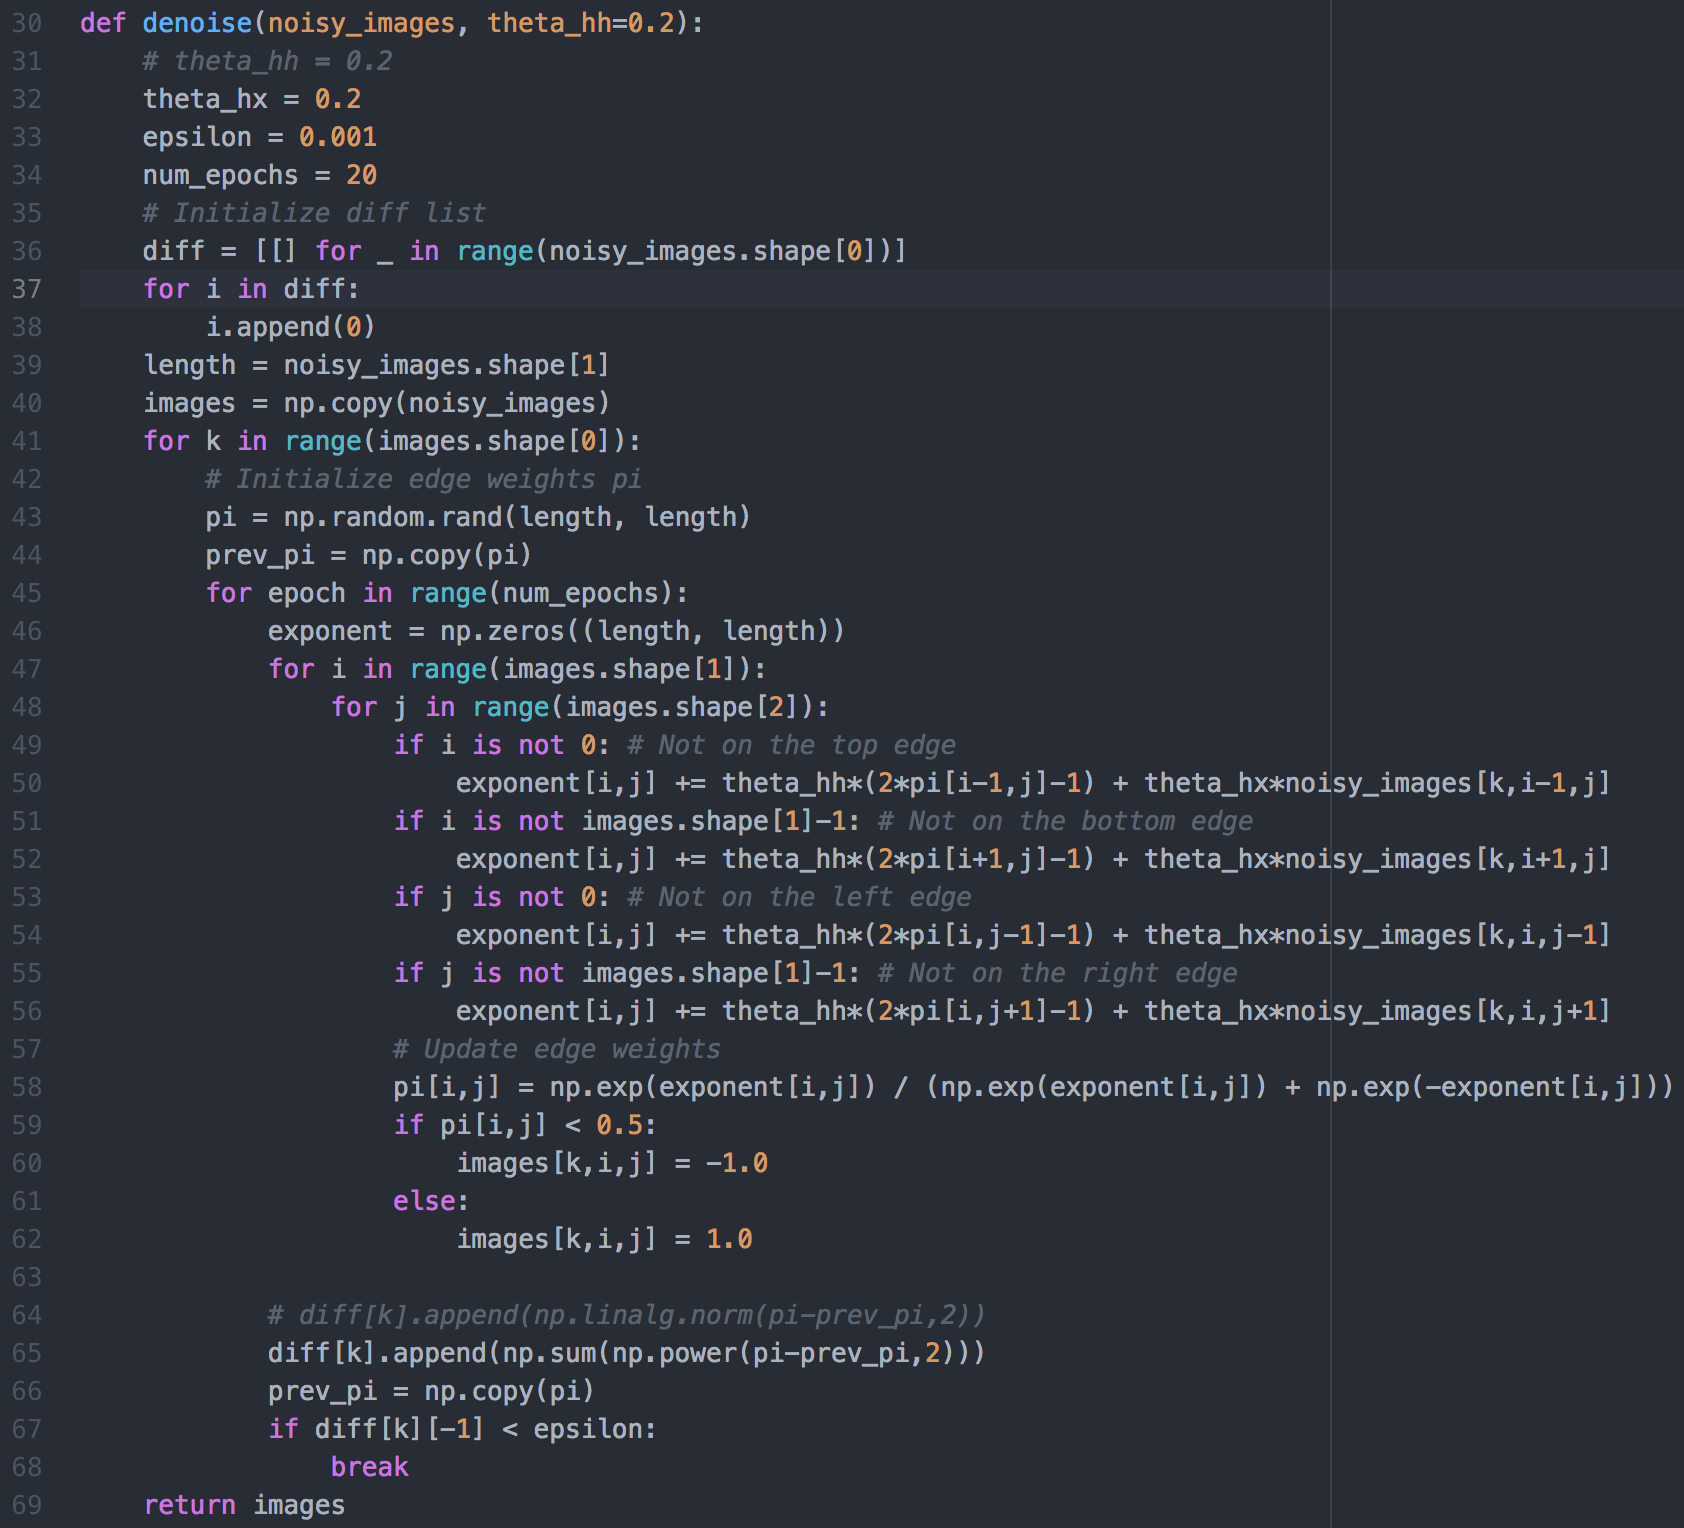
\includegraphics[width=0.95\textwidth]{2.png}
\end{figure}
\begin{figure}[H]
\centering
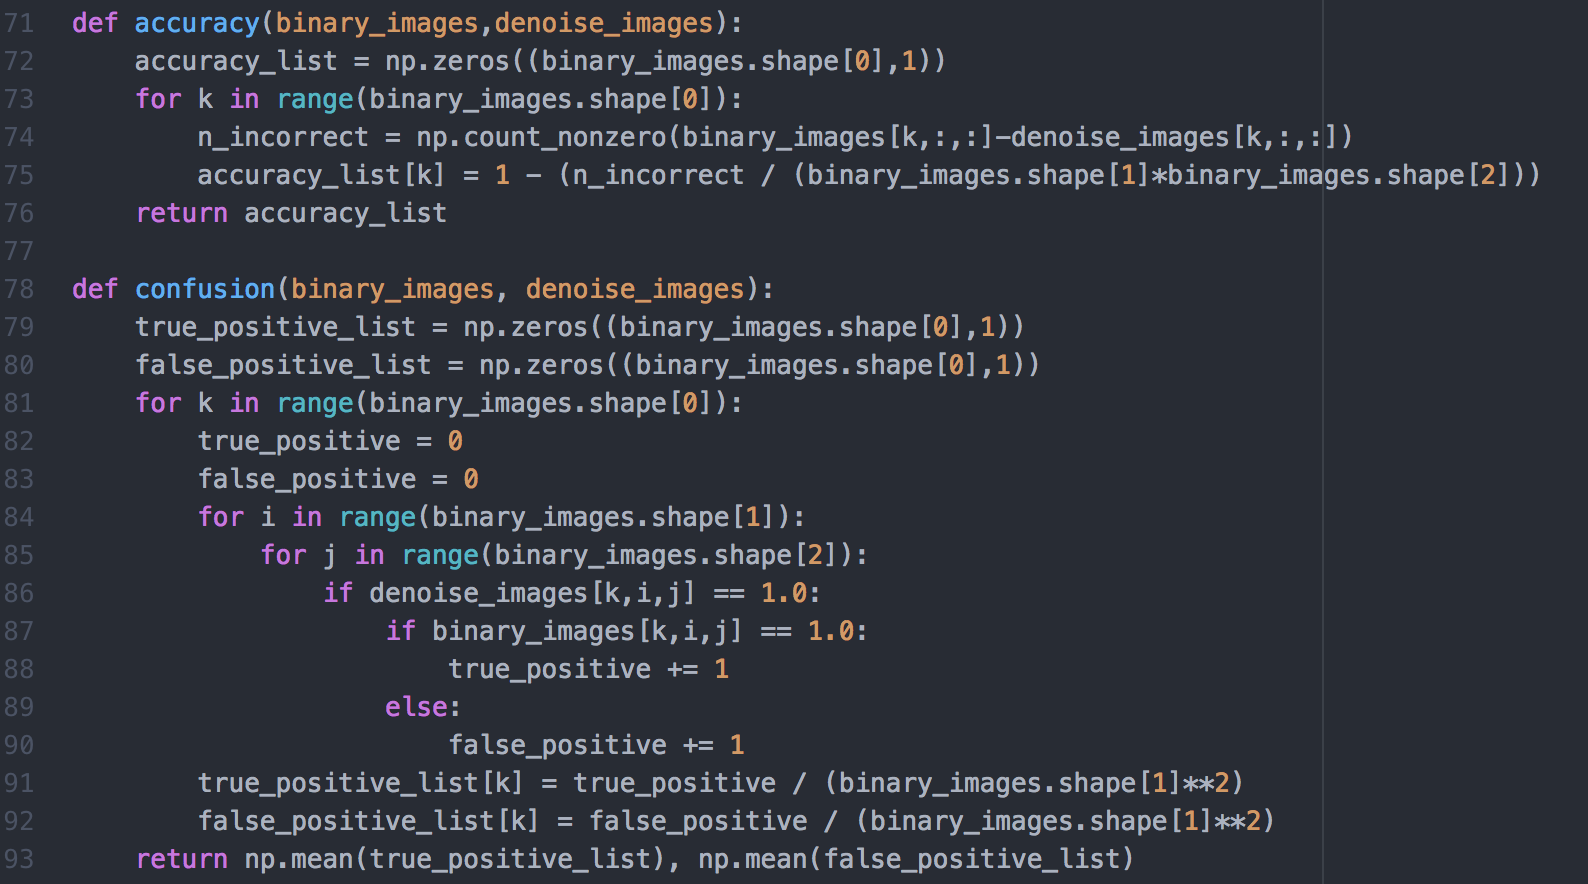
\includegraphics[width=0.95\textwidth]{3.png}
\end{figure}
\subsection{Main function}
\begin{figure}[H]
\centering
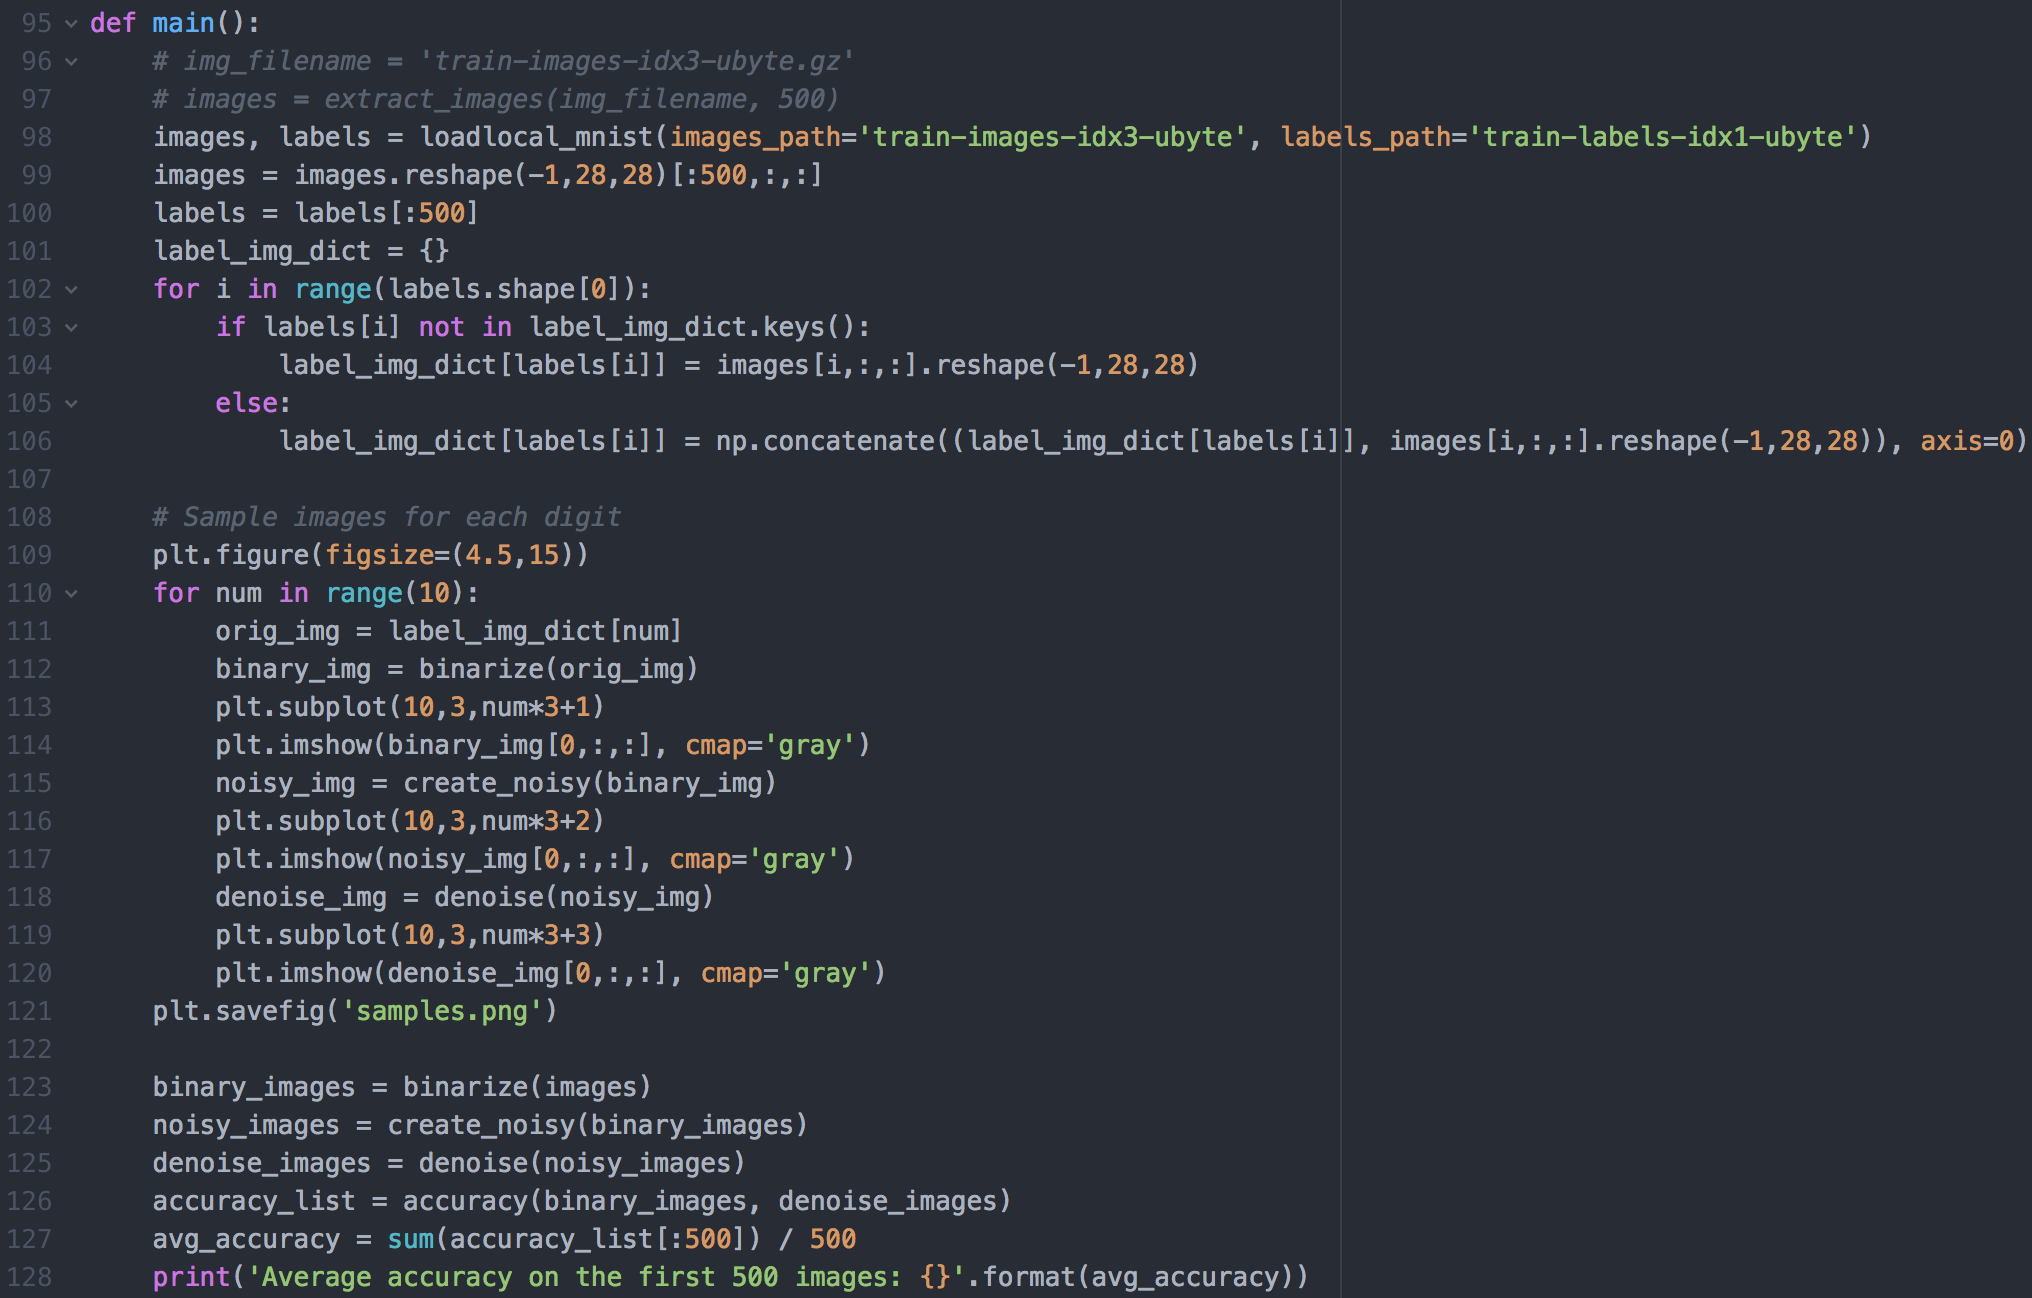
\includegraphics[width=0.95\textwidth]{4.png}
\end{figure}
\begin{figure}[H]
\centering
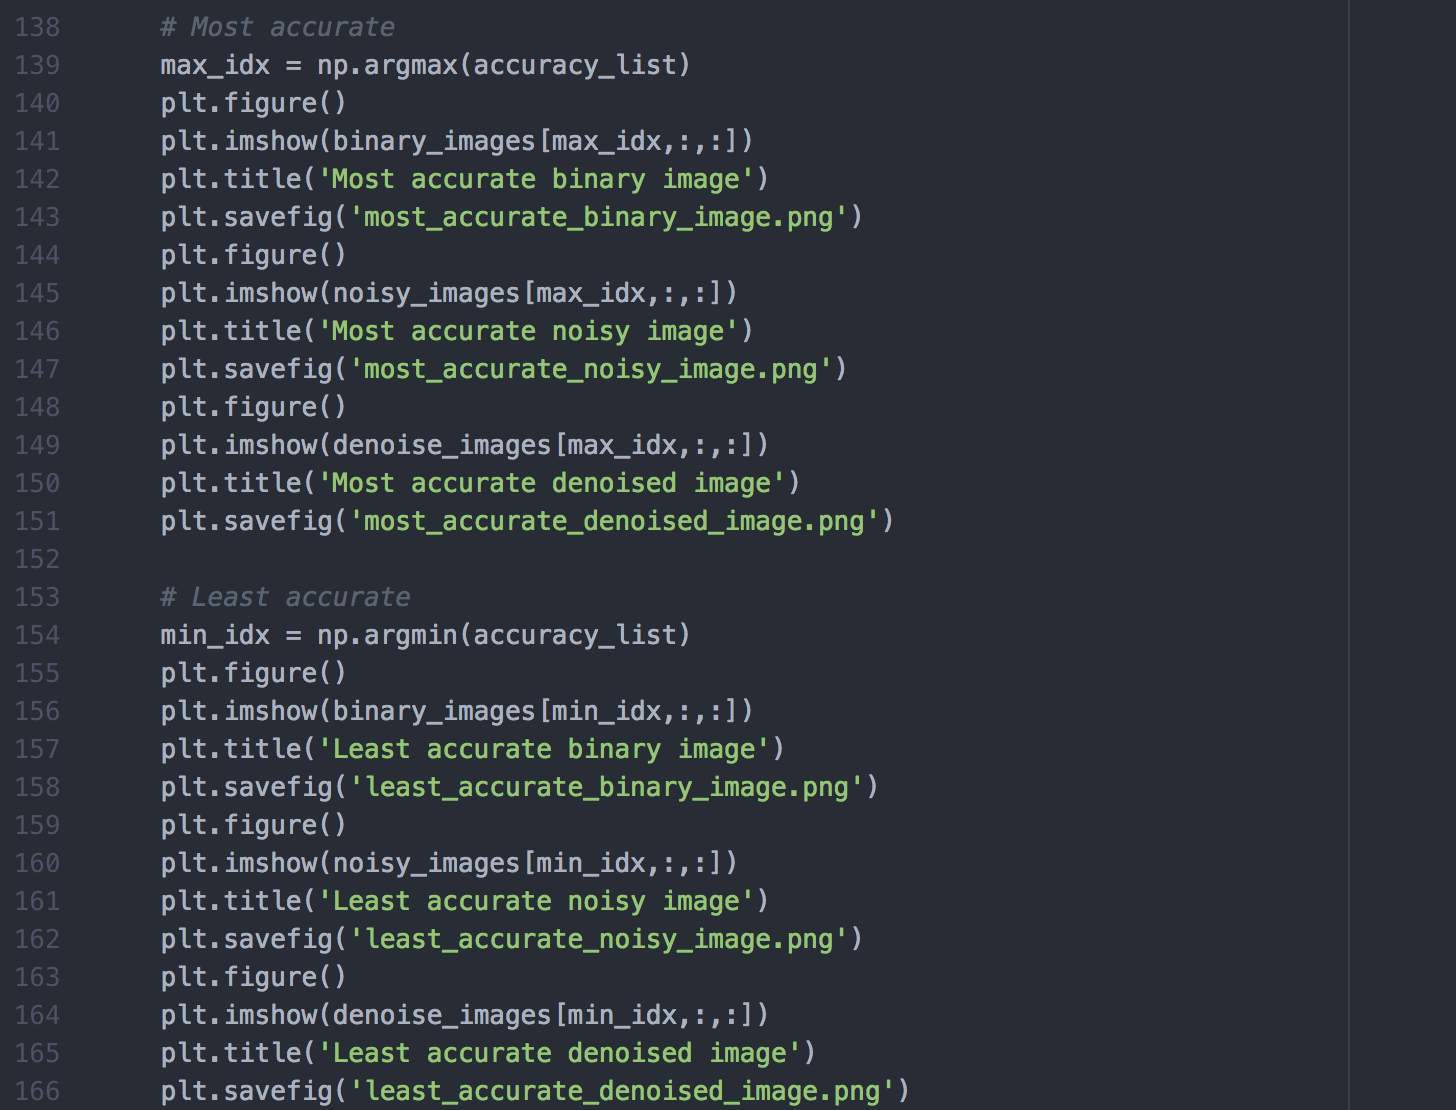
\includegraphics[width=0.95\textwidth]{5.png}
\end{figure}
\begin{figure}[H]
\centering
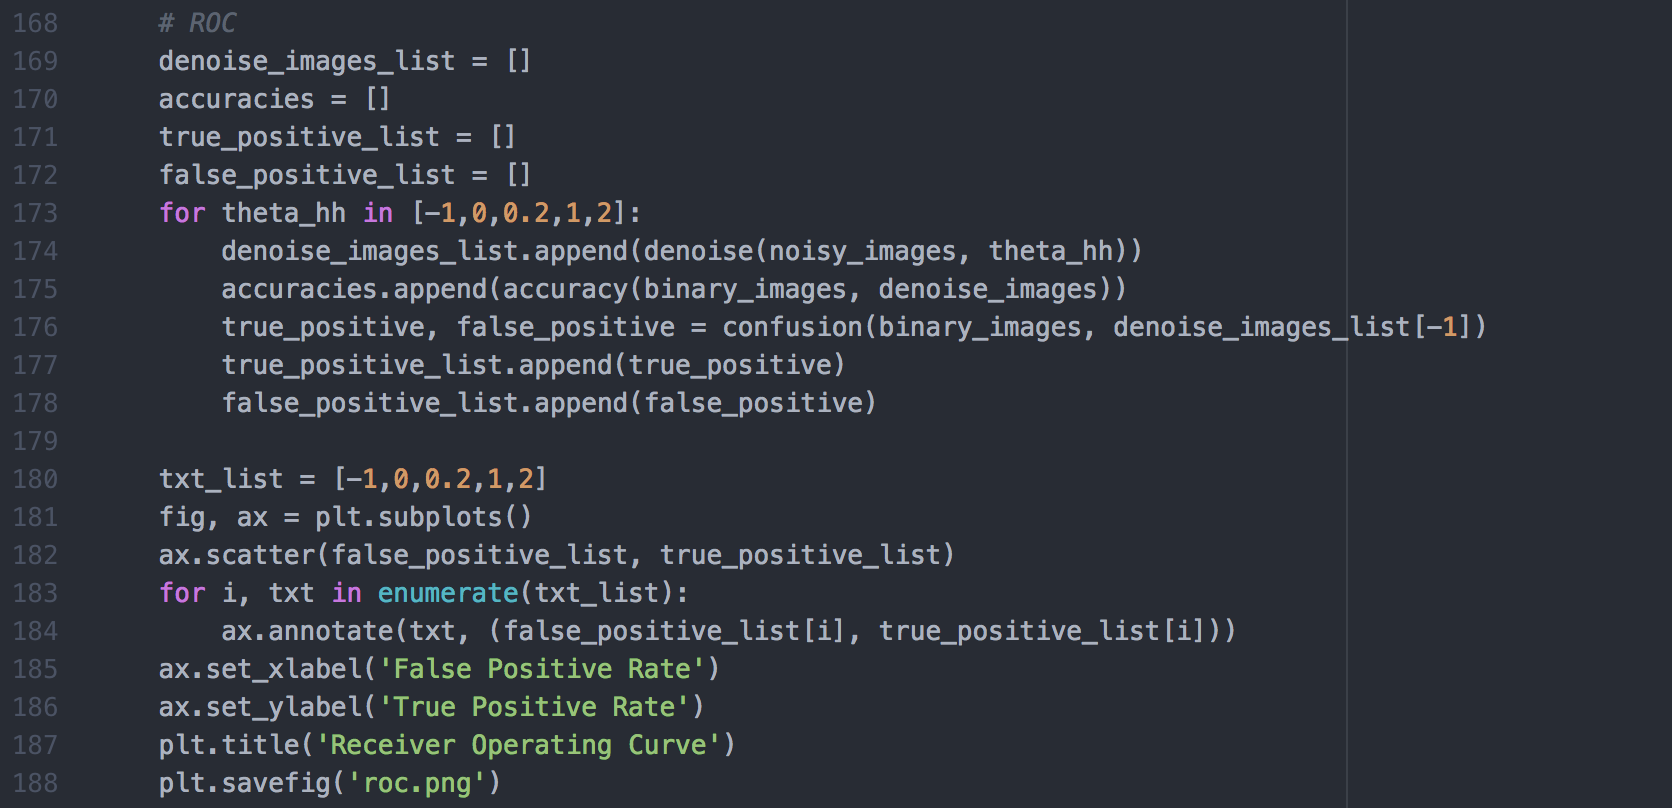
\includegraphics[width=0.95\textwidth]{6.png}
\end{figure}

\end{document}